\documentclass[10pt]{article}
\usepackage[russian]{babel}
\usepackage[utf8]{inputenc}
\usepackage[T2A]{fontenc}
\usepackage{graphicx}
\usepackage[export]{adjustbox}
\graphicspath{ {./images/} }

\title{САНКТ-ПЕТЕРБУРГСКИЙ ПОЛИТЕХНИЧЕСКИЙ УНИВЕРСИТЕТ ПЕТРА ВЕЛИКОГО }

\author{}
\date{}


\begin{document}
\maketitle
\section*{ИКНиК}
Лабораторная работа 12

«Телекоммуникационные технологии»

\section*{Выполнил:}
студент гр. 5130901/10101

Тучков Д.А.

(подпись)

Преподаватель:

Богач Н. В.

(подпись)

Санкт-Петербург

GNU Radio - это бесплатный набор инструментов для разработки программного обеспечения с открытым исходным кодом, который предоставляет блоки обработки сигналов для реализации программных радиомодулей. Его можно использовать с легкодоступным недорогим внешним радиочастотным оборудованием для создания программно-определяемых радиостанций или без оборудования в среде, подобной моделированию. Он широко используется в исследованиях, промышленности, научных кругах, правительстве и среди любителей для поддержки как исследований в области беспроводной связи, так и реальных радиосистем.\\
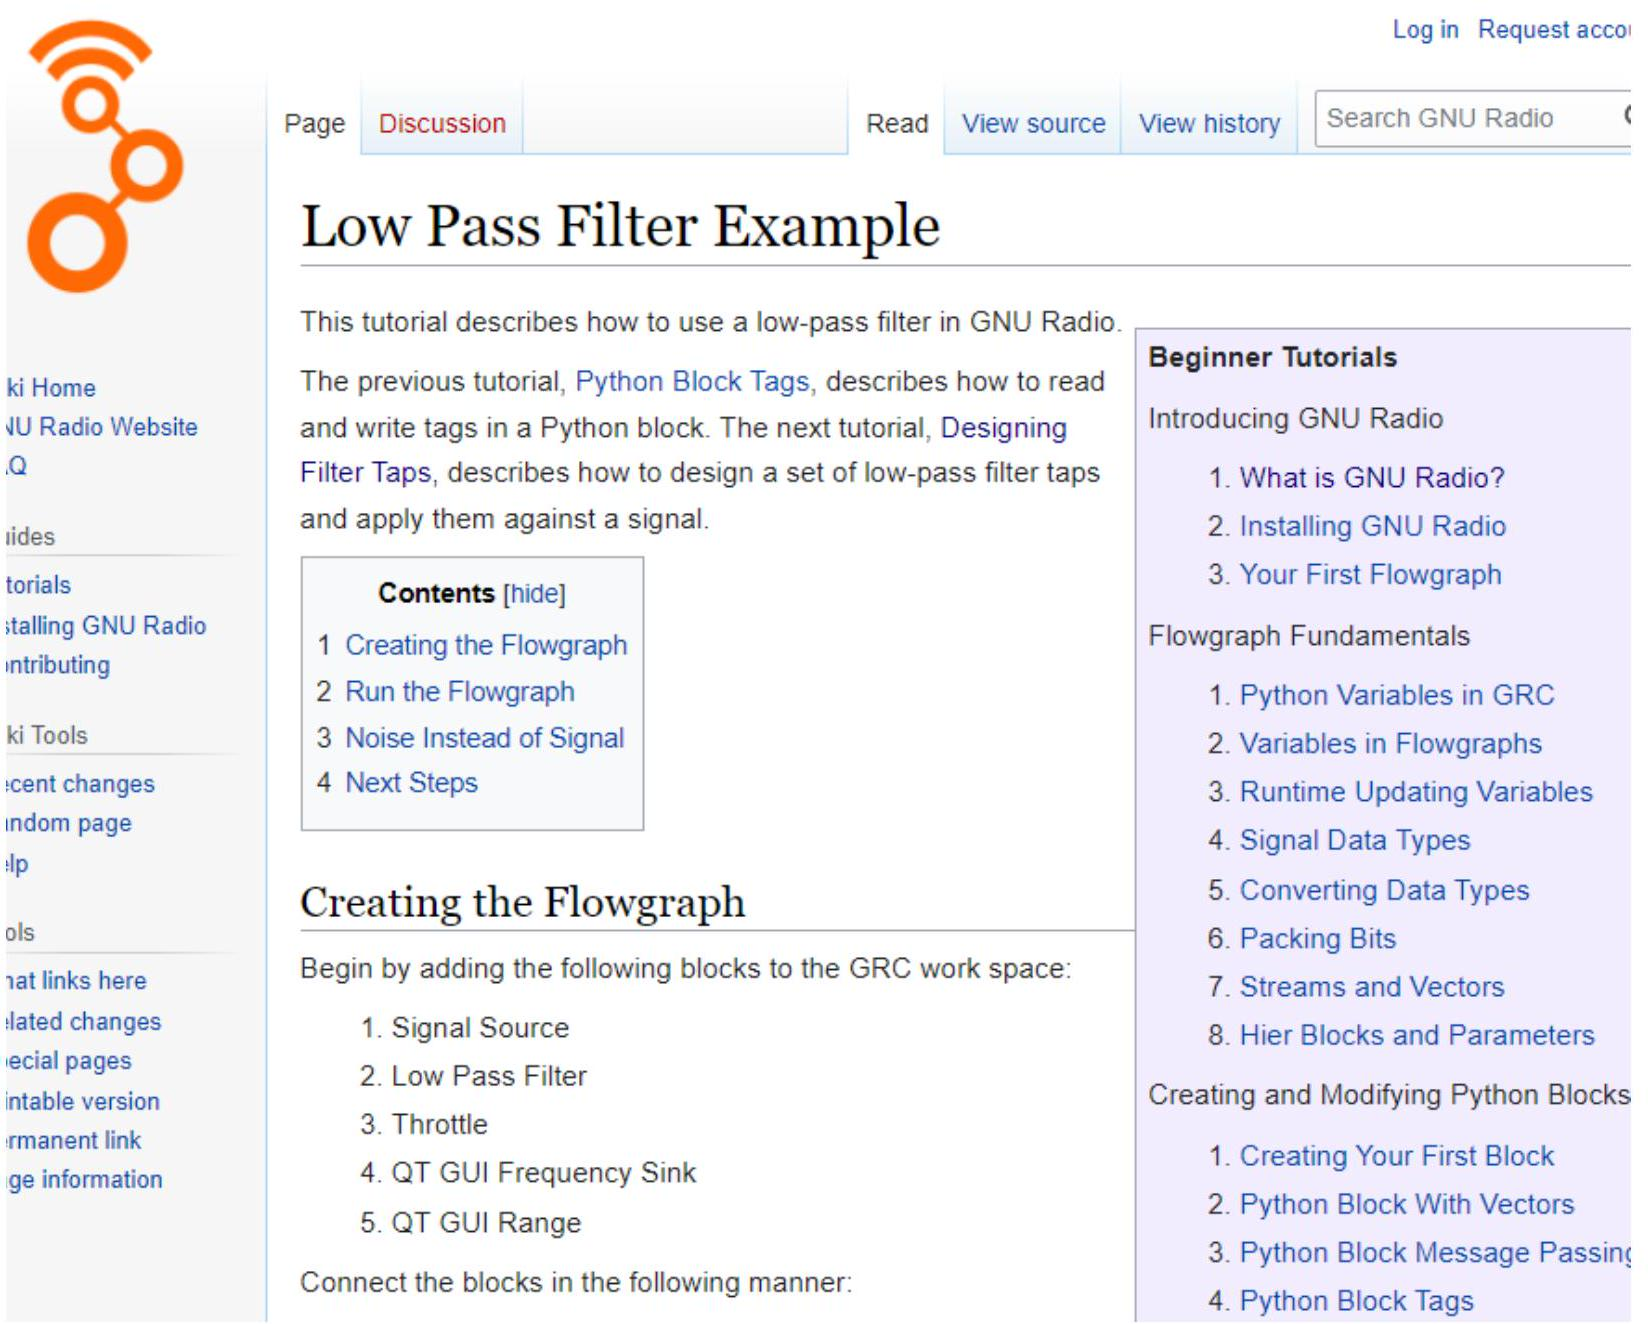
\includegraphics[max width=\textwidth, center]{motoda}

\section*{Фильтр нижних частот}
Создадим блок - графа

\begin{enumerate}
  \item Источник сигнала

  \item Фильтр нижних частот

  \item Дроссель

  \item Приемник частоты QT GUI

  \item Диапазон графического интерфейса QT

\end{enumerate}

\begin{center}
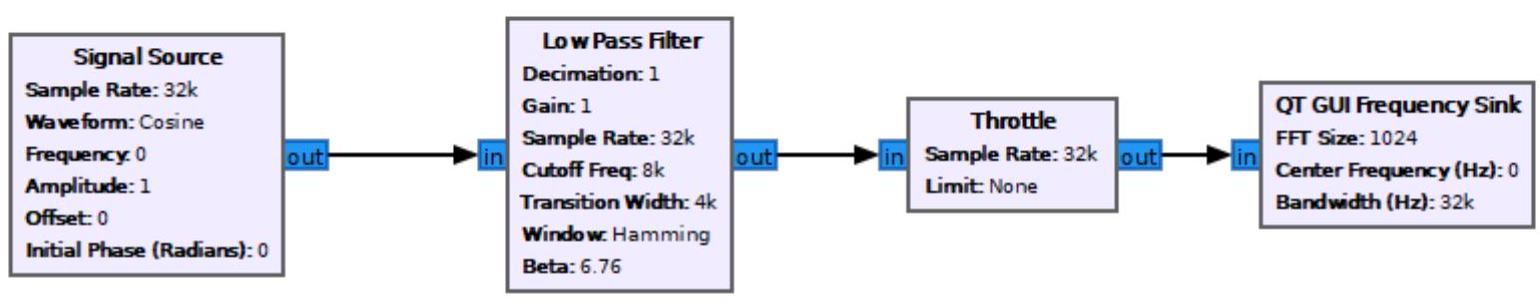
\includegraphics[max width=\textwidth]{cxema}
\end{center}

Блок QT GUI Range используется для управления частотой блока источника сигнала . Изменим свойства блока

\begin{itemize}
  \item Идентификатор: частота

  \item Значение по умолчанию: 0

  \item Начало: -samp\_rate/2

  \item Стоп: samp\_rate/2

\end{itemize}

\begin{center}
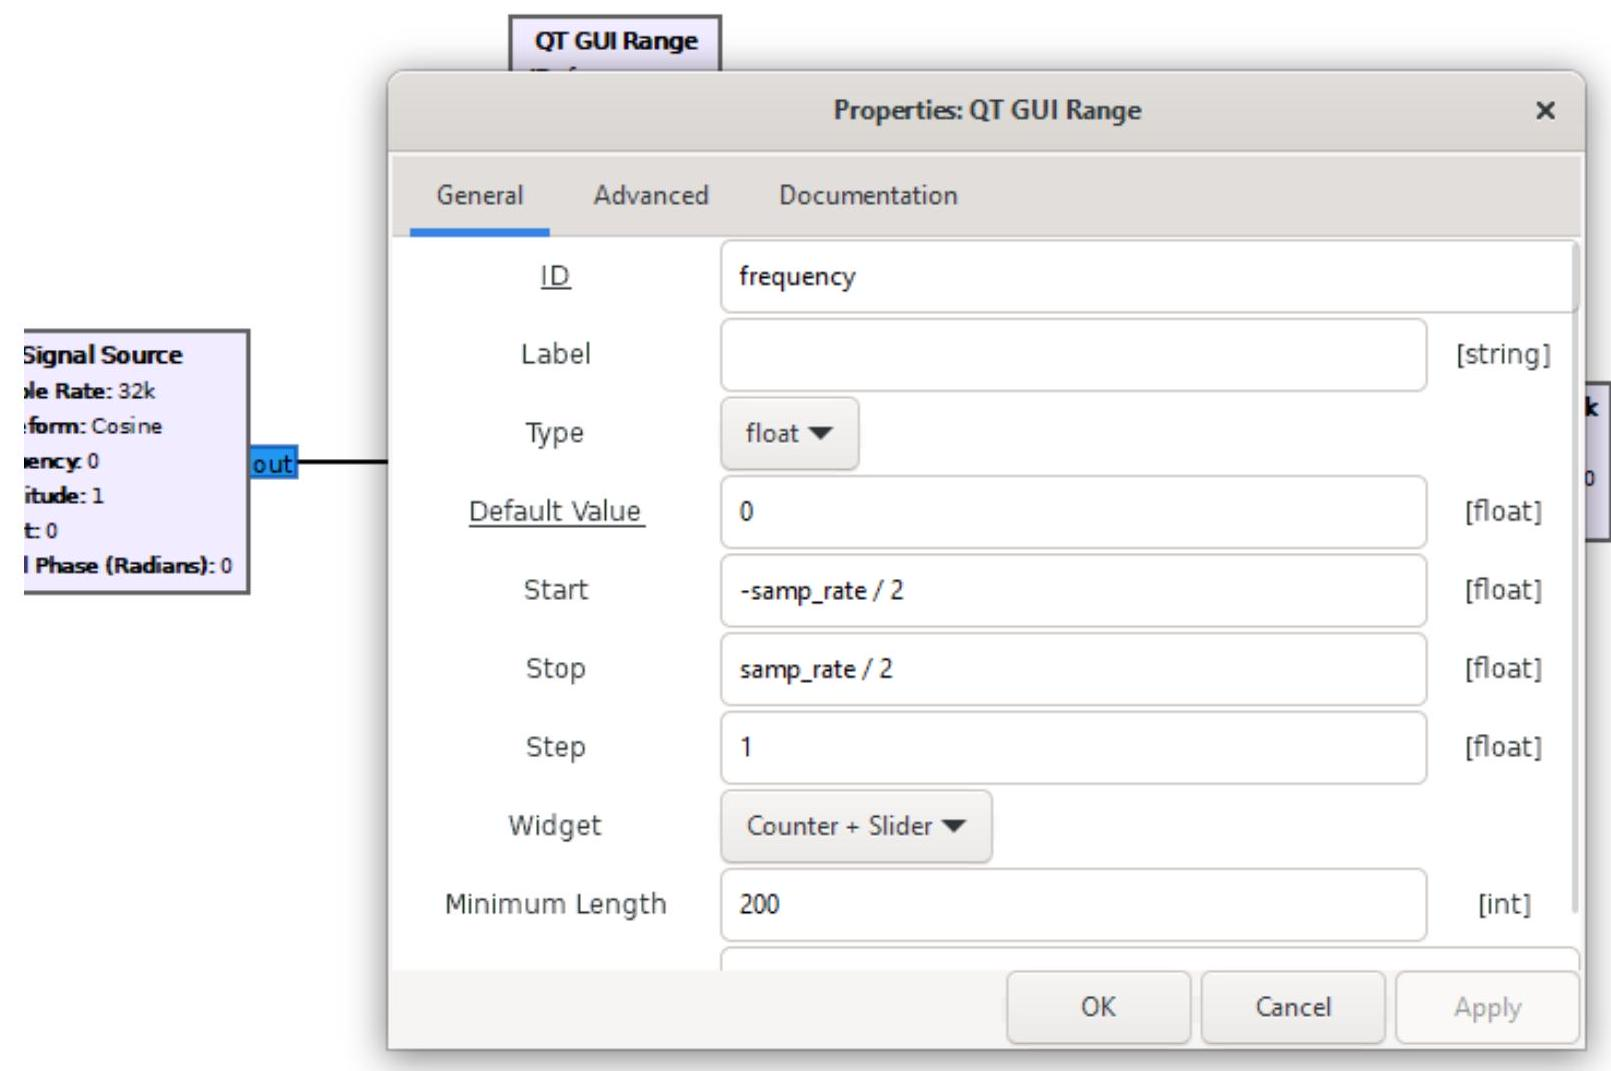
\includegraphics[max width=\textwidth]{QT}
\end{center}

\section*{Изменим свойства Signal Source}
\begin{center}
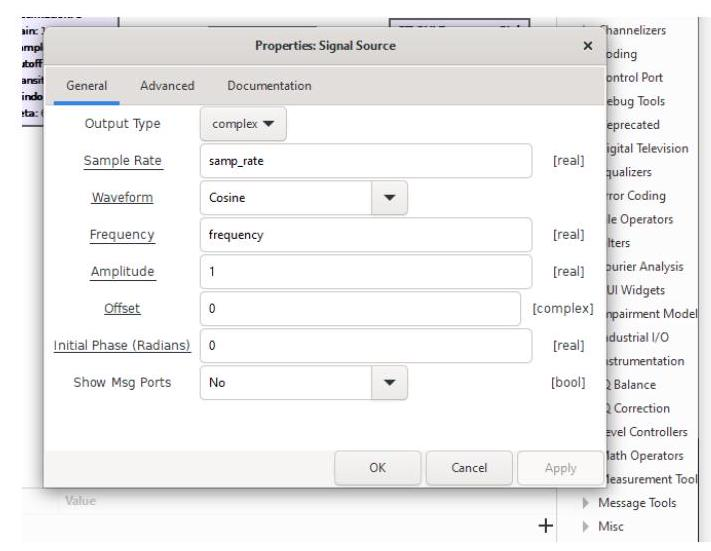
\includegraphics[max width=\textwidth]{signal}
\end{center}

Изменим свойства блока Low Pass Filter

\begin{itemize}
  \item Частота среза: samp\_rate/4
  \item Ширина перехода: samp\_rate/8
\end{itemize}

\begin{center}
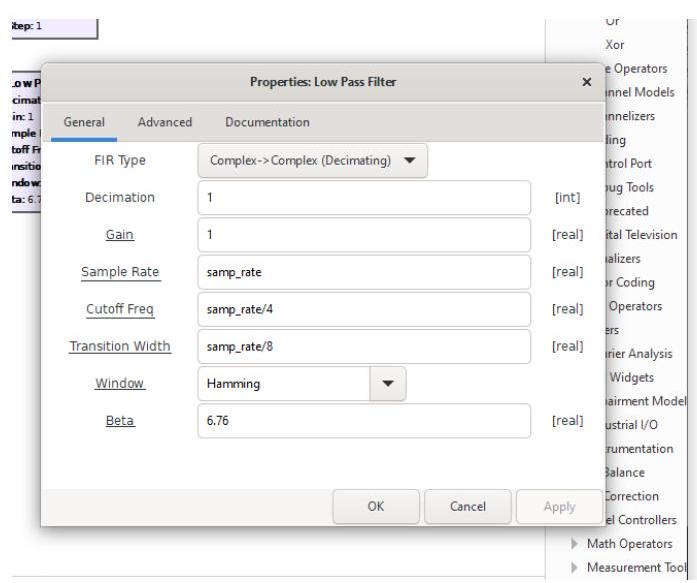
\includegraphics[max width=\textwidth]{low}
\end{center}

\section*{Запустим Блок-график}
\begin{center}
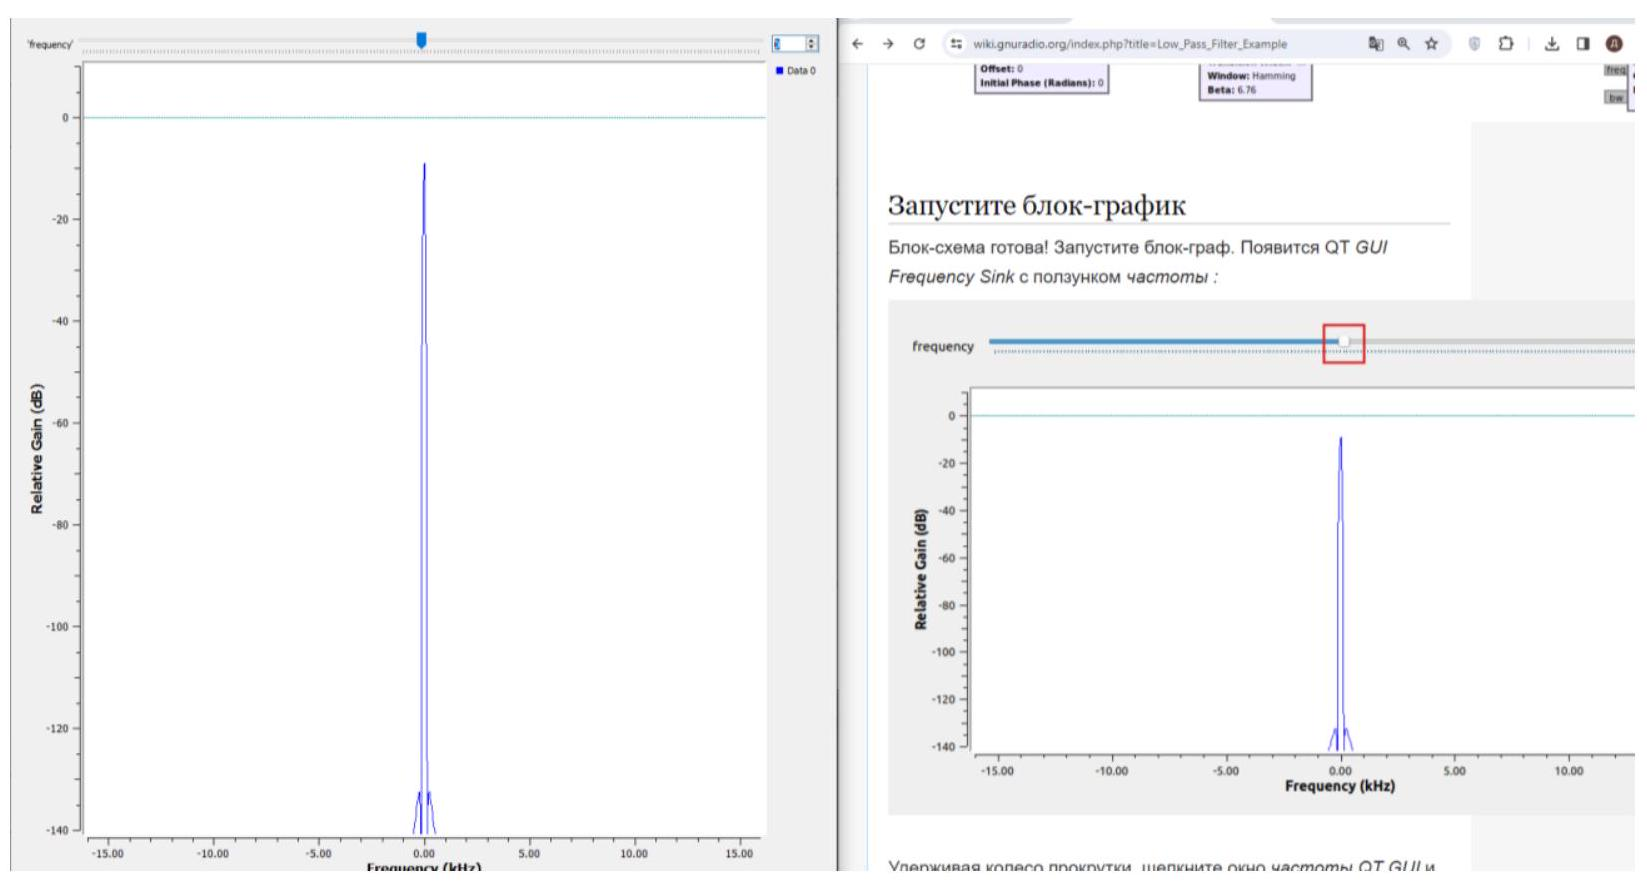
\includegraphics[max width=\textwidth]{launch}
\end{center}

\begin{center}
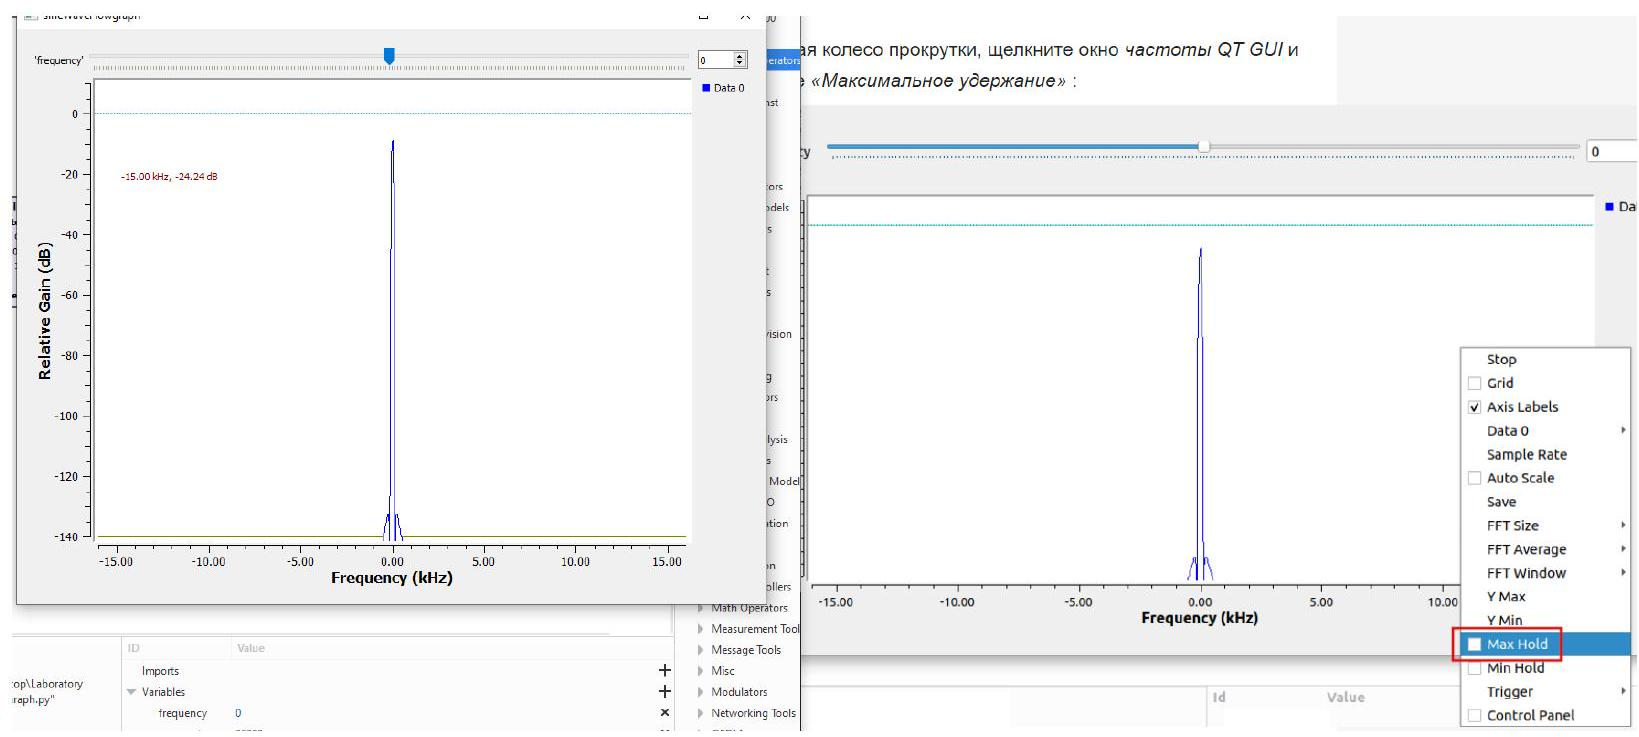
\includegraphics[max width=\textwidth]{max}
\end{center}

Опция Max Hold coxраняет и отображает максимальное значение на каждой частоте до тех пор, пока блок-график не будет закрыт.\\
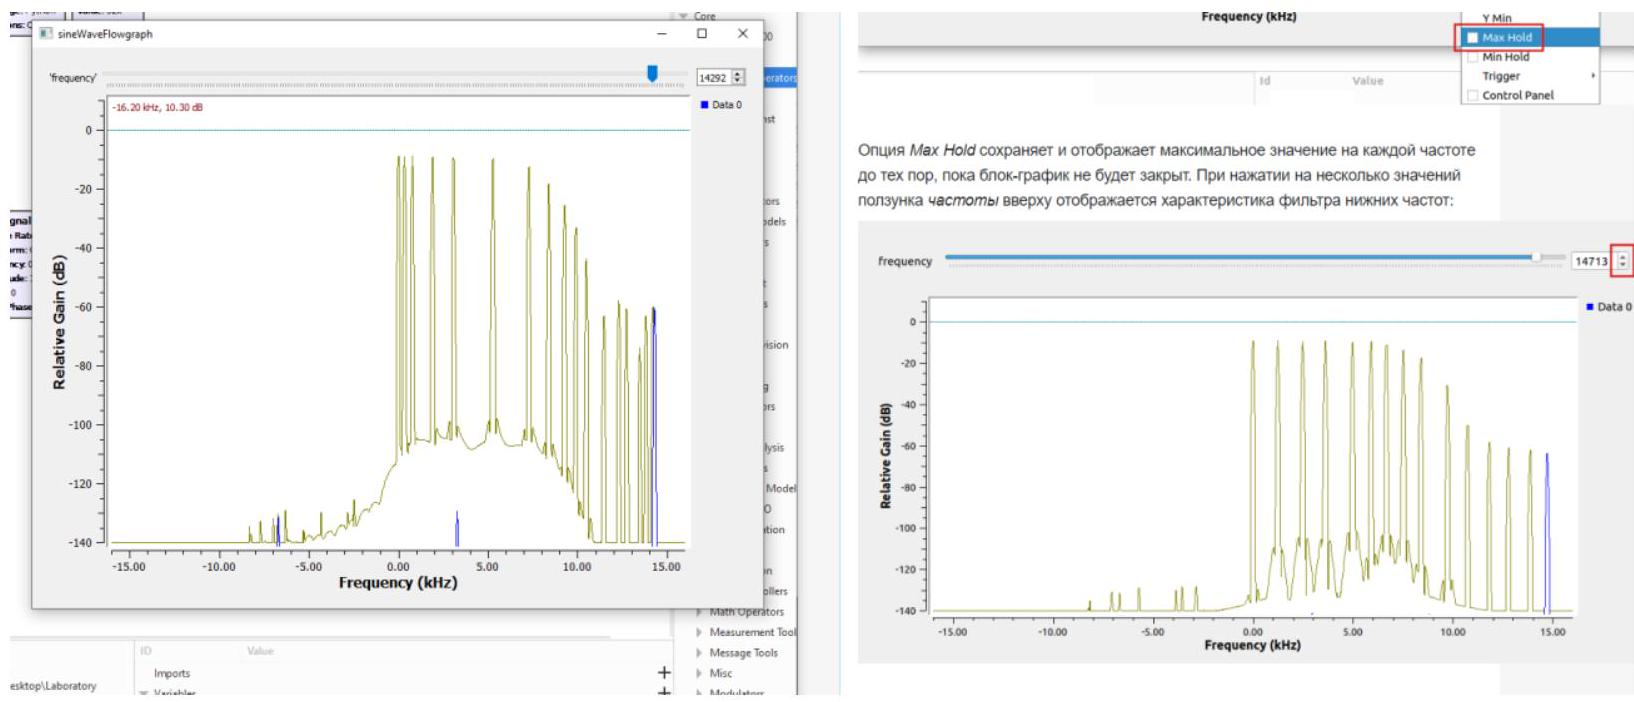
\includegraphics[max width=\textwidth, center]{save}

Опция Max Hold сохраняет и отображает максимальное значение на каждой частоте до тех пор, пока блок-график не будет закрыт. При нажатии на несколько значений ползунка частоты вверху отображается характеристика фильтра нижних частот:\\
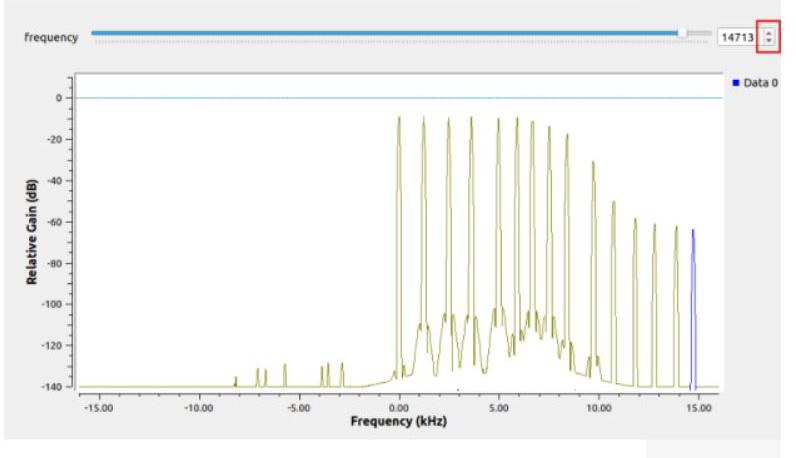
\includegraphics[max width=\textwidth, center]{graf}

Попробуем и другие настройки

MinHold

\begin{center}
\includegraphics[max width=\textwidth]{2024_03_24_25613617c1439d4099c5g-7}
\end{center}

\begin{center}
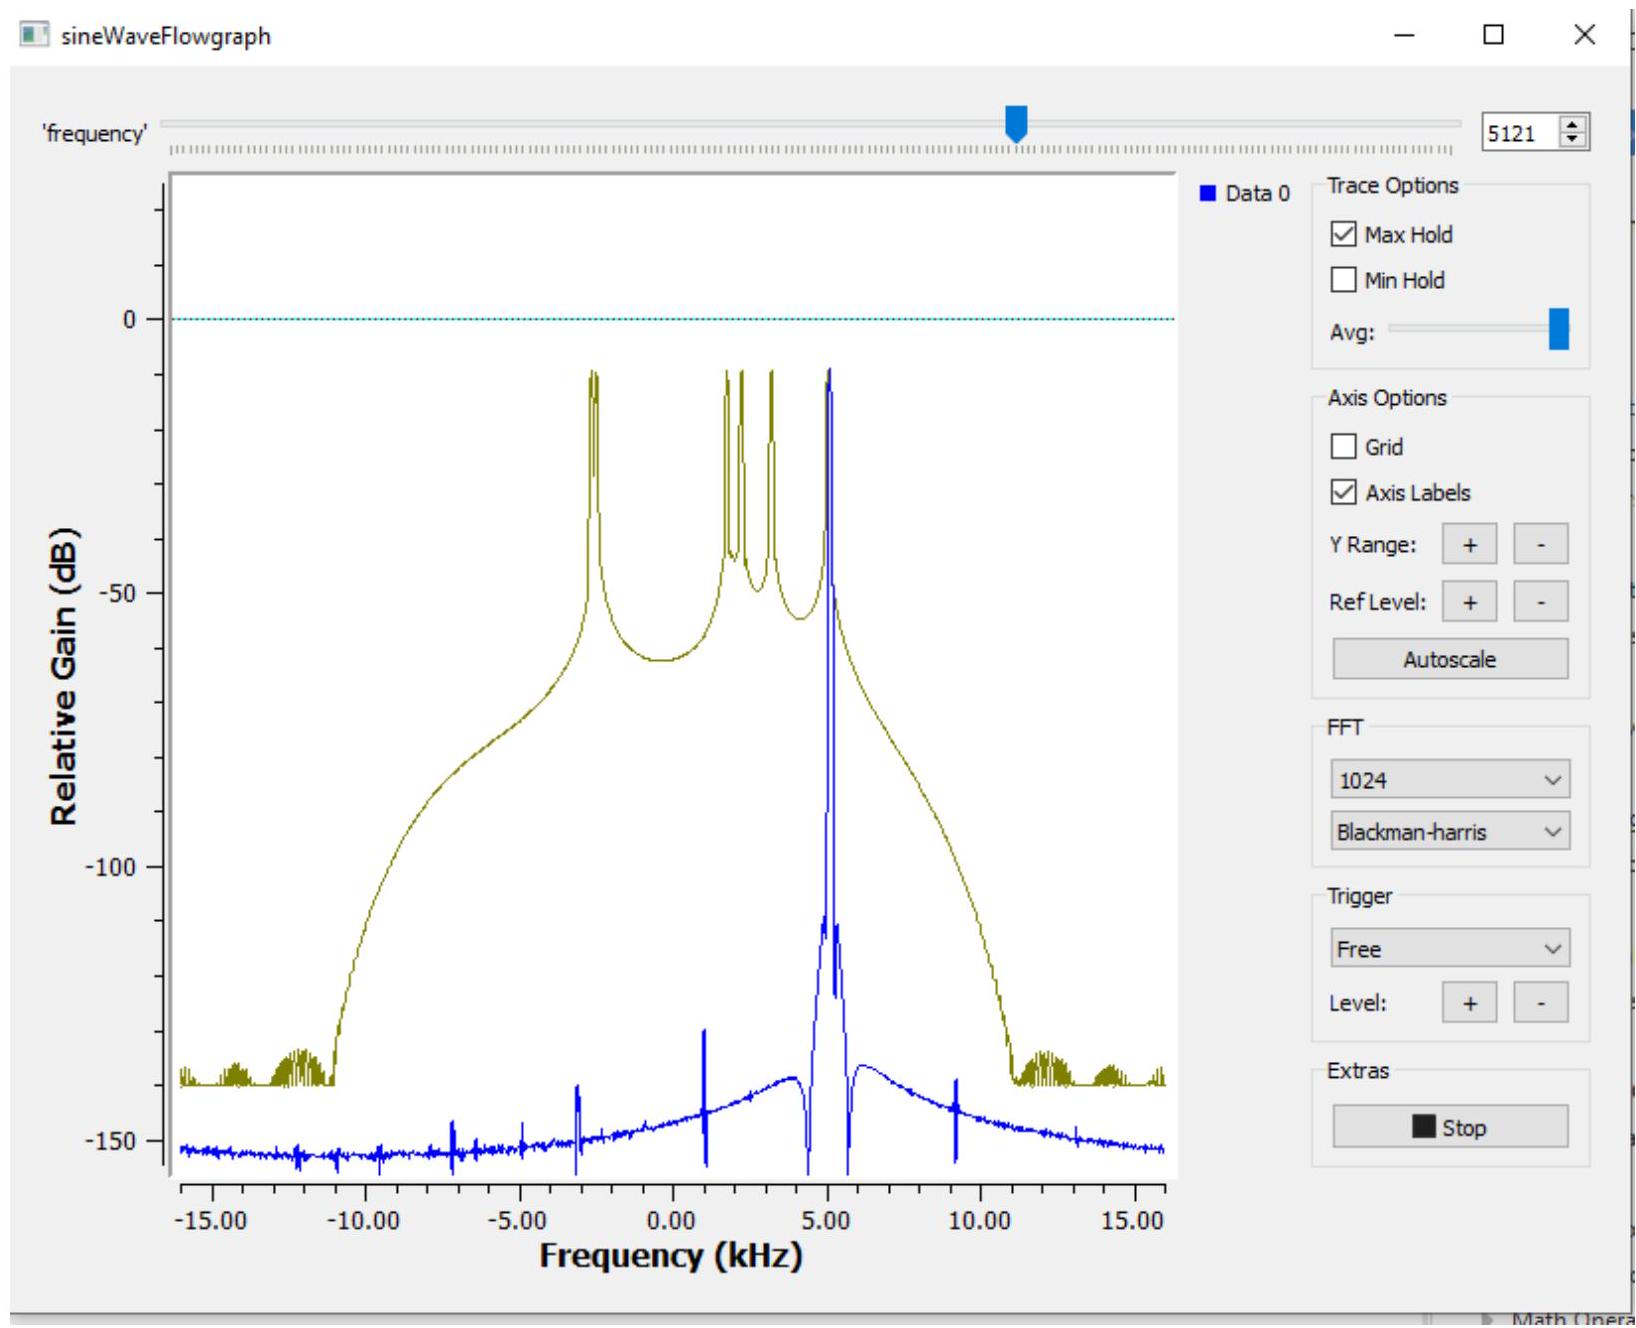
\includegraphics[max width=\textwidth]{MaxHold}
\end{center}


\end{document}